\documentclass[a4paper,11pt]{amsart}
\usepackage{amsmath}
\usepackage{amsthm,amsfonts,amssymb,graphics}
\usepackage{tikz}
\usetikzlibrary{patterns, calc, arrows.meta}

\begin{document}

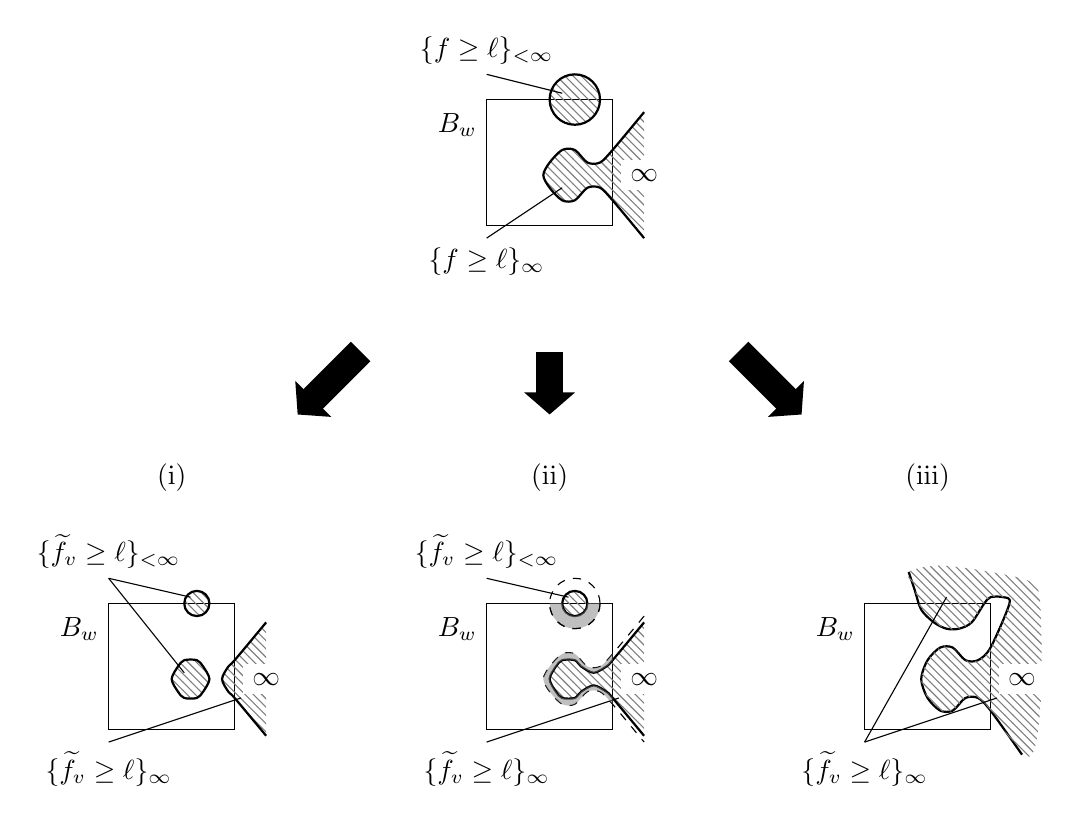
\begin{tikzpicture}[scale=0.8]
\draw (-1,-1) rectangle (1,1);
\node[left] at (-1,0.6) {$B_w$};
\draw[thick,pattern=north west lines,pattern color=gray] plot [smooth,tension=0.5] coordinates {(3/2,0.8)(1,0.2)(0.8,0)(0.6,0)(0.4,0.2)(0.2,0.2)(0,0)(-0.1,-0.2)(0,-0.4)(0.2,-0.6)(0.4,-0.6)(0.6,-0.4)(0.8,-0.4)(1,-0.6)(3/2,-1.2)};
\node[fill=white] at (1.5,-0.2) {$\infty$};
\draw[thick,pattern=north west lines,pattern color=gray] (0.4,1)circle (0.4);
\node[below] at (-1,-1.2) {$\{f\geq\ell\}_\infty$};
\draw (-1,-1.2)--(0.2,-0.4);
\node[above] at (-1,1.4) {$\{f\geq\ell\}_{<\infty}$};
\draw (-1,1.4)--(0.2,1.1);

\draw[-{Triangle[width=18pt,length=8pt]}, line width=10pt](-3,-3) -- (-4,-4);
\draw[-{Triangle[width=18pt,length=8pt]}, line width=10pt](0,-3) -- (0,-4);
\draw[-{Triangle[width=18pt,length=8pt]}, line width=10pt](3,-3) -- (4,-4);


\begin{scope}[shift={(-6,-8)}]
\node at (0,3) {(i)};
\draw (-1,-1) rectangle (1,1);
\node[left] at (-1,0.6) {$B_w$};

\draw[thick,pattern=north west lines,pattern color=gray] (0.4,1)circle (0.2);
\draw[thick,pattern=north west lines,pattern color=gray] plot [smooth,tension=0.5] coordinates {(3/2,0.7)(1,0.1)(0.9,0)(0.8,-0.2)(0.9,-0.4)(1,-0.5)(3/2,-1.1)};
\draw[thick,pattern=north west lines,pattern color=gray] plot [smooth cycle,tension=0.5] coordinates {(0.6,-0.2)(0.5,0)(0.4,0.1)(0.2,0.1)(0.1,0)(0,-0.2)(0.1,-0.4)(0.2,-0.5)(0.4,-0.5)(0.5,-0.4)};
\node[fill=white] at (1.5,-0.2) {$\infty$};
\node[below] at (-1,-1.2) {$\{\widetilde{f}_v\geq\ell\}_\infty$};
\draw (-1,-1.2)--(1.1,-0.5);
\node[above] at (-1,1.4) {$\{\widetilde{f}_v\geq\ell\}_{<\infty}$};
\draw (-1,1.4)--(0.3,1.1);
\draw (-1,1.4)--(0.2,-0.1);
\end{scope}


\begin{scope}[shift={(0,-8)}]
\draw (-1,-1) rectangle (1,1);
\node[left] at (-1,0.6) {$B_w$};
\node at (0,3) {(ii)};

\draw[dashed] plot [smooth,tension=0.5] coordinates {(3/2,0.8)(1,0.2)(0.8,0)(0.6,0)(0.4,0.2)(0.2,0.2)(0,0)(-0.1,-0.2)(0,-0.4)(0.2,-0.6)(0.4,-0.6)(0.6,-0.4)(0.8,-0.4)(1,-0.6)(3/2,-1.2)};
\draw[dashed] (0.4,1)circle (0.4);

\draw[thick,pattern=north west lines,pattern color=gray] (0.4,1)circle (0.2);
\draw[thick,pattern=north west lines,pattern color=gray] plot [smooth,tension=0.5] coordinates {(3/2,0.7)(1,0.1)(0.9,0)(0.7,-0.1)(0.5,0)(0.4,0.1)(0.2,0.1)(0.1,0)(0,-0.2)(0.1,-0.4)(0.2,-0.5)(0.4,-0.5)(0.5,-0.4)(0.7,-0.3)(0.9,-0.4)(1,-0.5)(3/2,-1.1)};
\node[fill=white] at (1.5,-0.2) {$\infty$};
\node[below] at (-1,-1.2) {$\{\widetilde{f}_v\geq\ell\}_\infty$};
\draw (-1,-1.2)--(1.1,-0.5);
\node[above] at (-1,1.4) {$\{\widetilde{f}_v\geq\ell\}_{<\infty}$};
\draw (-1,1.4)--(0.3,1.1);

\clip (-1,-1) rectangle (1,1);
\fill[color=gray,opacity=0.5] plot [smooth,tension=0.5] coordinates {(3/2,0.8)(1,0.2)(0.8,0)(0.6,0)(0.4,0.2)(0.2,0.2)(0,0)(-0.1,-0.2)(0,-0.4)(0.2,-0.6)(0.4,-0.6)(0.6,-0.4)(0.8,-0.4)(1,-0.6)(3/2,-1.2)(3/2,-1.1)(1,-0.5)(0.9,-0.4)(0.7,-0.3)(0.5,-0.4)(0.4,-0.5)(0.2,-0.5)(0.1,-0.4)(0,-0.2)(0.1,0)(0.2,0.1)(0.4,0.1)(0.5,0)(0.7,-0.1)(0.9,0)(1,0.1)(3/2,0.7)};

\draw ($(1,2)+(90:0.6)$)arc (90:450:0.4);
\fill[color=gray,opacity=0.5] ($(0.4,1)+(90:0.4)$)arc (90:450:0.4)--($(0.4,1)+(450:0.2)$) arc(450:90:0.2);
\draw[dashed] (0.4,1)circle (0.4);
\end{scope}





\begin{scope}[shift={(6,-8)}]
\draw (-1,-1) rectangle (1,1);
\node[left] at (-1,0.6) {$B_w$};
\node at (0,3) {(iii)};

\draw[thick] plot [smooth,tension=0.5] coordinates {(-0.3,1.5)(-0.2,1.2)(-0.1,0.9)(0.1,0.7)(0.3,0.6)(0.5,0.6)(0.7,0.7)(0.9,1)(1,1.1)(1.2,1.1)(1.3,1)(1,0.3)(0.8,0.1)(0.6,0.1)(0.4,0.3)(0.2,0.3)(0,0.1)(-0.1,-0.2)(0,-0.5)(0.2,-0.7)(0.4,-0.7)(0.6,-0.5)(0.8,-0.5)(1,-0.7)(3/2,-1.4)};

\fill[pattern=north west lines,pattern color=gray] plot [smooth cycle,tension=0.5] coordinates {(-0.3,1.5)(-0.2,1.2)(-0.1,0.9)(0.1,0.7)(0.3,0.6)(0.5,0.6)(0.7,0.7)(0.9,1)(1,1.1)(1.2,1.1)(1.3,1)(1,0.3)(0.8,0.1)(0.6,0.1)(0.4,0.3)(0.2,0.3)(0,0.1)(-0.1,-0.2)(0,-0.5)(0.2,-0.7)(0.4,-0.7)(0.6,-0.5)(0.8,-0.5)(1,-0.7)(3/2,-1.4)(1.7,-1.3)(1.8,-0.5)(1.8,0.7)(1.7,1.3)(1,1.5)(0.2,1.6)};

\node[fill=white] at (1.5,-0.2) {$\infty$};
\node[below] at (-1,-1.2) {$\{\widetilde{f}_v\geq\ell\}_\infty$};
\draw (-1,-1.2)--(1.1,-0.5);
\draw (-1,-1.2)--(0.3,1.1);

\end{scope}
\end{tikzpicture}

\end{document}